\textbf{مورد استفاده:}
ورود
\\
\textbf{شرح مختصر :UC}
در این قسمت مهمان وارد سایت می‌شود و به عنوان کاربر شناخنه می‌شود.
\\
\textbf{پيش شرط:}
عضویت.
\\
\textbf{سناريو اصلی:}
\begin{enumerate}
\item
شروع
\item
مهمان دکمه ورود را انتخاب می‌کند و سیستم فرم ورود را به مهمان نمایش می‌دهد.
\item
مهمان فرم ورود را تکمیل می‌کند و با دکمه ارسال، فرم تکمیل شده را به سیستم ارسال می‌کند.
\item
سیستم فرم ورود را بررسی می‌کند و اطلاعات را از بانک اطلاعات دریافت می‌کند.
\item
کاربر در سایت شناسایی و وارد می‌شود.
\item
پایان
\end{enumerate}

\noindent
\textbf{پس شرط:}
ندارد.
\\
\textbf{سناريوهای فرعی:}
\\
\textbf{سناريو فرعی 1:}
خطا در اطلاعات فرم ورود
\\
\textbf{شرح مختصر :UC}
این سناریو در مرحله ۴ سناریو اصلی در صورت خطا در اطلاعات فرم ورود اجرا می‌شود.
\begin{enumerate}
\item
شروع
\item
اطلاعات فرم بررسی می‌شود و خطاها مشخص می‌شوند.
\item
یک پیغام به مهمان نمایش داده می‌شود و درخواست اصلاح اطلاعات فرم را دارد.
\item
از مرحله 3 سناریو اصلی ادامه پیدا می‌کند.
\item
پایان
\end{enumerate}

\noindent
\textbf{سناريو فرعی 2:}
کاربر با موفقیت وارد می‌شود.
\\
\textbf{شرح مختصر :UC}
این سناریو در مرحله ۴ سناریو اصلی در صورت موفقیت آمیز بودن ورود اجرا می‌شود.
\begin{enumerate}
\item
شروع
\item
اطلاعات فرم بررسی می‌شود و یک پیغام به کاربر نمایش داده می‌شود که ورود موفقیت آمیزی داشته.
\item
از مرحله 5 سناریو اصلی ادامه پیدا می‌کند.
\item
پایان
\end{enumerate}

\noindent
\textbf{سناريو فرعی 3:}
کاربر وجود ندارد.
\\
\textbf{شرح مختصر :UC}
این سناریو در مرحله ۴ سناریو اصلی در صورت وجود نداشتن اطلاعات در بانک اطلاعات اجرا می‌شود.
\begin{enumerate}
	\item
	شروع
	\item
	اطلاعات فرم بررسی می‌شود و وجود نداشتن کاربر مشخص می‌شوند.
	\item
	یک پیغام به مهمان نمایش داده می‌شود و دکمه ثبت‌نام نمایش داده می‌شود.
	\item
	پایان
\end{enumerate}

\noindent
\textbf{پس شرط:}
ندارد .

\begin{figure}[H]
	\centering
	\includegraphics[width=1\textwidth]{Diagram/2.Activity/ورود.jpg}
	\caption{دیاگرام فعالیت ورود}
	\label{fig:a:ورود}
\end{figure}
\begin{figure}[H]
	\centering
	\includegraphics[width=1\textwidth]{Diagram/3.Sequence/ورود.jpg}
	\caption{دیاگرام توالی ورود}
	\label{fig:s:ورود}
\end{figure}
\begin{figure}[H]
\centering
\includegraphics[width=1\textwidth]{Diagram/4.Collaboration/ورود.jpg}
\caption{دیاگرام همکار ورود}
\label{fig:c:ورود}
\end{figure}
